\documentclass{article}

\usepackage{graphicx, amsmath}

\begin{document}

\title{Ordinal Data clustering and prediction}

\author{Quan Zhao}

\maketitle

% \begin{abstract}
% \textbf{If you need an abstract, then it goes here. While you are reading this document, please also criticise it for the writing style, grammar, consistency, suitability, etc. }
% \end{abstract}

% 1. Search for relevant literature - 0:30
% 2. Evaluate and select sources -  0:58
% 3. Identify themes, debates, and gaps - 1:26
% 4. Outline your literature review's structure - 1:56
% 5. Write it - 2:34

\section{Introduction}
% introduction of the research topic
% (1/2 to 1 page).

% Finite mixture models are a flexible and powerful tool in statistical analysis, offering several key features that contribute to their widespread use in various fields.  These models assume that the observed data are generated from a combination of different probability distributions, each representing a distinct subpopulation within the overall population. The term "finite" in finite mixture models refers to the specific number of components or subpopulations in the mixture.

% Figure~\ref{fig:trend} shows the finite mixture modelling has strong trend in publications.

% intro of Ordinal Data

\subsection*{Ordinal Data}

Ordinal data is a type of categorical data in statistics that represents categories with a meaningful order or ranking among them, but without a precise difference in the scale between each category. This type of data is distinct because, while it allows for a rank order among the values, the intervals between the values are not necessarily equal or known. This means that ordinal data can tell us about the order of categories but not about the magnitude of difference between them.

Ordinal data include, Ranking data which can be sorted or ranked in order, but the distances between data points are not meaningful.
Ordinal data often consists of labels or descriptions, though it can be coded with numbers for analysis. Even when numerical codes are used, arithmetic operations (such as addition or subtraction) are not meaningful.
Statistical analysis of ordinal data typically involves non-parametric methods. The median and mode can be used as measures of central tendency

Ordinal data is common in surveys, questionnaires, and other forms of qualitative research, where it's used to capture attitudes, opinions, preferences, and other subjective assessments that inherently have an order but not a measurable distance between categories. 

Ordinal data are the most frequently encountered type of data in the social
sciences. Survey data, in which respondents are asked to characterize their opinions
on scales ranging from “strongly disagree” to “strongly agree,” are a common
example of such data. For our purposes, the defining property of ordinal data
is that there exist a clear ordering of the response categories, but no underlying
interval scale between them. For example, it is generally reasonable to assume an
ordering of the form
strongly disagree < disagree < dont know < agree < strongly agree,
but it usually does not make sense to assign integer values to these categories.
Thus, statements of the type
\[
\text{``disagree''} - \text{``strongly disagree''}
\]

\[
\text{``agree''} - \text{``don't know''}
\]
are not assumed. (Johnson, 2006~/cite{johnson2006ordinal})

% clustering

\subsection*{Ordinal Data Clustering}

Finite mixture models have emerged as a versatile and powerful statistical tool, garnering increasing attention across various scientific and research disciplines. These models, predicated on the assumption that observed data arise from a blend of several probability distributions, each representing a distinct subpopulation, have revolutionized our approach to understanding complex data structures. The designation "finite" in finite mixture models is pivotal, indicating the specific, but variable, number of components or subgroups within the data. This finite aspect offers a balance between model complexity and interpretability, allowing for detailed yet manageable analysis of diverse datasets.

The significance of finite mixture models is vividly illustrated in Figure~\ref{fig:trend}, which showcases a robust upward trajectory in related publications. This trend not only reflects the growing academic and practical interest in these models but also underscores their evolving sophistication and broadening applicability. From the early advancements in maximizing likelihood estimation through algorithms like EM, as pioneered by McLachlan in 2000, to the more recent developments in handling a variety of data types, including binary, count, and ordinal data, finite mixture models have continuously adapted and expanded their scope.

\begin{figure}[ht!] % 'h!' places the figure here, in the text
    \centering % Centers the figure
    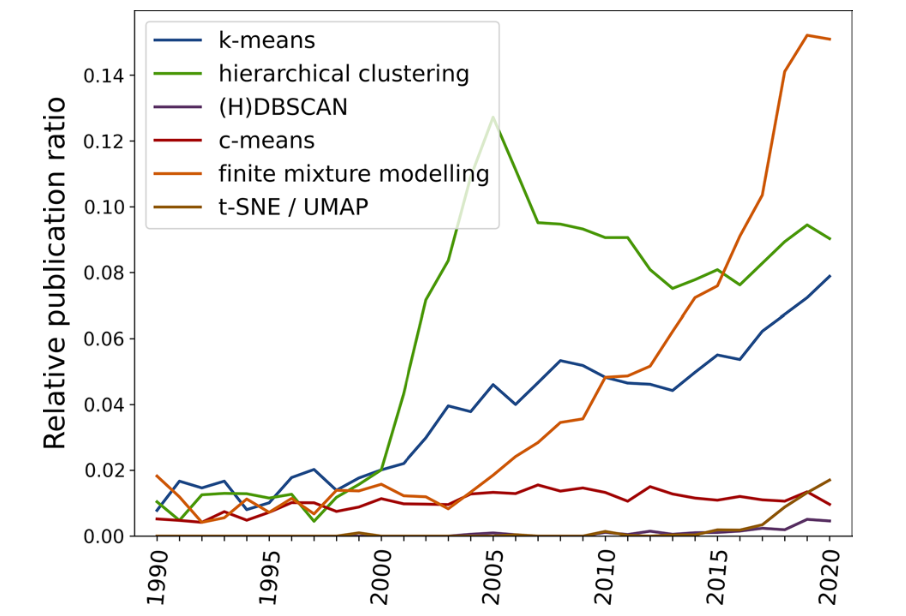
\includegraphics[width=0.6\textwidth]{images/trend.png} % Include the image with 50% of the text width
    \caption{The increase in publications indexed by PubMed that mention a keyword specific to cluster analyses relative to the number of publications 
    that mention a traditional statistical test. 
    Particularly sharp increases can be seen for finite mixture modelling.
    From~\cite{dalmaijer2022statistical}.} % Caption for the image
    \label{fig:trend} % Label for referencing the figure in the text
  \end{figure}


\section{literature review}
% The section on analysis is split into two sub-sections. 
% (about 2-3 pages)

% In 2000~\cite{mclachlan2000finite} proposesed the mixture model in terms of $Y_j$ and $Z_j$ is most useful 
% in that it allws the the maximum likelihood estimate (MLE) of the Mixture distribution to be computed via 
% a straightforward application of the EM algorithms.
% It is also useful in implementing the MCMC methods in the fitting of mixture models in a Bayesian framework.
% (here, $Y_j$ is feature vector and $Z_j$ is components label vector.)

% In 2002~\cite{figueiredo2002unsupervised} proposes an unsupervised algorithm for learning a finite mixture model from multivariate data. The algorithm can select the number of components and does not require careful initialization, making it less sensitive to initialization than the standard expectation-maximization algorithm. The proposed method also avoids the possibility of convergence toward a singular estimate at the boundary of the parameter space. The authors provide a formal and principled approach to clustering and model selection, which can be applied to a wide range of unsupervised learning problems. The paper is well-written and provides a clear explanation of the proposed algorithm, making it a valuable resource for researchers and practitioners in the field of machine learning.

% In 2010~\cite{10.1214/09-SS053} addresses key issues in estimation, model selection, and likelihood maximization using the EM algorithm, offering practical guidance for researchers and practitioners. this work also provide valuable insights into methodologies for simulating realizations from Gaussian mixture models, graphical tools for visual representation, and applications involving non-Gaussian mixtures. 

% In 2016~\cite{matechou2016biclustering} proposes finite mixture models that can simultaneously cluster the rows and columns of two-mode ordinal categorical response data. The models utilize the popular proportional odds parameterization and provide insights into major patterns present in the data. Model-fitting is performed using the EM algorithm, resulting in a fuzzy allocation of rows and columns to corresponding clusters. The clustering ability of the models is evaluated through simulation studies and demonstrated using two real data sets. The paper addresses the challenge of modeling heterogeneity in two-mode ordinal data by developing finite mixture models that offer a comprehensive and interpretable approach to clustering both rows and columns, ultimately providing insights into the major patterns present in the data.

% In 2016~\cite{fernandez2016mixture} introduces a new methodology for clustering rows and columns in a matrix of ordinal data. It utilizes likelihood-based methods through finite mixtures with the stereotype model. The paper demonstrates the reliability of this approach through a simulation study and further illustrates its application with two examples. Additionally, it reviews and compares several model choice measures, providing a robust framework for analyzing ordinal data matrices using fuzzy clustering techniques.

% In 2018~\cite{jacques2018model} introduces a novel model-based co-clustering algorithm for ordinal data, which leverages the latent block model and the BOS distribution. The BOS model, a type of mixture model, is employed to probabilistically model the ordinal data. Notably, the algorithm's parsimony and interpretability are underscored, along with its capability to handle missing data, a crucial aspect in mixture model applications. The authors provide a comprehensive description of the algorithm, including its inference strategy and tools for selecting the number of co-clusters. Furthermore, the paper presents numerical studies and real data applications to demonstrate the efficiency and practical relevance of the proposed model. Overall, this work contributes significantly to the field of clustering algorithms for ordinal data, offering a valuable tool for practitioners working with high-dimensional datasets and showcasing the potential of mixture models in this context.

% In 2019~\cite{fernandez2019finite} improved their work. It extends the finite mixture models to a broader range of data types, including binary, count, and ordinal data, under a unified statistical framework. It also introduces maximum likelihood estimation parameters and the option of using likelihood information criteria for model comparison. and it presentation of a Bayesian approach, where parameters and the number of clusters are estimated simultaneously. 

%

% Mixture models have evolved significantly since McLachlan's 2000 proposition of using $Y_j$ and $Z_j$ for efficient maximum likelihood estimation (MLE) through the EM algorithm. This method not only simplified MLE computations but also laid the groundwork for Bayesian approaches using MCMC methods in mixture models (McLachlan, 2000~\cite{mclachlan2000finite}).

% In 2002, Figueiredo's unsupervised algorithm marked a paradigm shift by autonomously determining the number of components in a finite mixture model. This innovation reduced the dependency on careful initialization, a common pitfall in earlier methods, and addressed the issue of singular estimates (Figueiredo, 2002~\cite{figueiredo2002unsupervised}).

% A decade later, the 2010 paper by Volodymyr and Ranjan offered comprehensive guidelines for EM algorithm applications in mixture models, addressing estimation, model selection, and maximization challenges. This work also expanded the field's understanding of non-Gaussian mixtures and introduced graphical tools for better visualization and simulation (Volodymyr and Ranjan, 2010~\cite{10.1214/09-SS053}).

% The subsequent years saw an expansion into biclustering via finite mixture models, particularly for two-mode ordinal categorical data. Matechou in 2016 used proportional odds parameterization to cluster data rows and columns, offering a nuanced approach to understanding data patterns (Matechou, 2016~\cite{matechou2016biclustering}). Fernandez in the same year provided an alternative clustering methodology through likelihood-based finite mixtures, showcasing its effectiveness in handling ordinal data (Fernandez, 2016~\cite{fernandez2016mixture}).

% Jacques' 2018 contribution is particularly notable for introducing a model-based co-clustering algorithm that effectively handles ordinal data using the BOS distribution. This method's capacity to manage missing data and its parsimonious approach marked a significant advancement in mixture model applications (Jacques, 2018~\cite{jacques2018model}).

% Finally, Fernandez's 2019 paper extended the scope of finite mixture models to encompass binary, count, and ordinal data, showcasing the versatility of these models. This work also highlighted the Bayesian approach for simultaneous estimation of parameters and cluster numbers, reflecting the field's ongoing evolution towards more sophisticated and comprehensive models (Fernandez, 2019~\cite{fernandez2019finite}).

%

\subsection*{Early Developments (2000--2010)}

McLachlan's 2000 paper marked a crucial step in mixture model applications by simplifying the maximum likelihood estimation (MLE) using the EM algorithm. This approach, utilizing $Y_j$ and $Z_j$, not only enhanced the computational efficiency of MLE but also laid a foundational strategy for Bayesian approaches and MCMC methods in mixture models. The paper’s impact is evident in its widespread adoption across various domains, from bioinformatics to finance, where mixture models are employed (McLachlan, 2000~\cite{mclachlan2000finite}).

In 2002, Figueiredo's introduction of an unsupervised algorithm for learning finite mixture models was a game-changer. This method's ability to autonomously select the number of components represented a significant leap over previous techniques, which often relied on arbitrary or manual component selection. Additionally, the algorithm's robustness against initialization issues and singular estimates made it a go-to choice for practitioners dealing with complex multivariate data (Figueiredo, 2002~\cite{figueiredo2002unsupervised}).

A key paper in 2010 by Volodymyr and Ranjan addressed practical challenges in applying the EM algorithm for mixture models. This comprehensive guide to estimation, model selection, and likelihood maximization was a boon for both researchers and practitioners. Notably, the work extended beyond Gaussian mixtures, offering insights and methodologies for simulating and visualizing non-Gaussian mixtures, thereby broadening the applicability of mixture models (Volodymyr and Ranjan, 2010~\cite{10.1214/09-SS053}).

\subsection*{Recent Developments (2010--2019)}

In 2016, Matechou's proposal of finite mixture models for biclustering two-mode ordinal categorical data introduced a novel approach to data analysis. By employing proportional odds parameterization, these models provided a nuanced understanding of complex data patterns, useful in fields such as genomics and social sciences where ordinal data is prevalent. The utilization of the EM algorithm for model-fitting underscored the enduring relevance of this method in mixture model applications (Matechou, 2016~\cite{matechou2016biclustering}).

Fernandez in 2016 offered an alternative methodology for clustering ordinal data. The use of likelihood-based methods through finite mixtures with the stereotype model presented a robust framework for analyzing complex data structures. This approach was particularly notable for its application in fuzzy clustering techniques, an area of growing interest in data science (Fernandez, 2016~\cite{fernandez2016mixture}).

Jacques' 2018 introduction of a model-based co-clustering algorithm was a significant advancement. The algorithm's ability to handle missing data and its interpretability made it especially relevant for high-dimensional datasets. The BOS distribution employed in this model underscored the continuous innovation in probabilistic modeling techniques, catering to the increasing complexity of data in modern research (Jacques, 2018~\cite{jacques2018model}).

Fernandez's 2019 extension of finite mixture models to binary, count, and ordinal data under a unified statistical framework represented a consolidation and expansion of mixture model applications. The introduction of maximum likelihood estimation parameters and the Bayesian approach for simultaneous estimation were indicative of the field's progression towards more flexible and comprehensive modeling techniques (Fernandez, 2019~\cite{fernandez2019finite}).

% \section{Conclusions}

% In summary, the evolution of infinite mixture models from 2000 to 2019 has largely concentrated on clustering, successfully categorizing new observations into predefined clusters. However, this predominant focus presents a fertile ground for future research. An intriguing direction is exploring models that dynamically adjust or create new cluster spaces as data evolves, moving beyond static clustering methods. Such developments could lead to more adaptive and flexible models, capable of handling the complexities of continuously changing data sets. The integration of mixture models with other advanced machine learning techniques might also offer novel approaches, potentially enhancing their applicability and effectiveness across various domains. This potential for innovation signifies a promising future for the field of infinite mixture models.

\section{Conclusion and Future Directions}

The evolution of mixture models from McLachlan's initial work in 2000 to advanced models in 2019 showcases a field marked by dynamic growth and innovation. These models have not only solved historical challenges but also set the stage for future advancements. As the field progresses, a key focus is integrating machine learning with traditional statistical methods, enhancing the capability of mixture models to accurately predict cluster membership for new data points. This is especially relevant in artificial intelligence applications, where mixture models contribute to improved pattern recognition and decision-making.

Furthermore, as data complexity and volume continue to escalate, the demand for robust, efficient, and versatile mixture models is more critical than ever. Future research is expected to concentrate on scaling up these models and improving their adaptability across diverse data types and structures. This progression underscores the mixture models' indispensable role in modern data analysis, poised to address the ever-growing challenges in data science and AI.

\bibliographystyle{plain}
\bibliography{bibliography} % Replace 'yourbibfile' with the name of your .bib file


\end{document}

